\documentclass[addpoints,12pt]{exam}
\newcommand{\ds}{\displaystyle}
\usepackage[margin=0.8in]{geometry}
\usepackage{subcaption}
\usepackage{tikz}
\usepackage{amssymb,amsmath,graphicx,wrapfig,verbatim,wasysym, enumitem,psfragx,color}
\usepackage{multicol}


\usepackage{pgf,tikz,pgfplots}
\usepackage{stmaryrd}
\usetikzlibrary{arrows, shapes.geometric, matrix, turtle, plotmarks}

%\usepackage{fancyhdr}
%\setlength{\headheight}{13.6pt}
%\pagestyle{fancy}
%\lhead{Math 222}
%\chead{ Midterm 1 }
%\rhead{Spring 2022}

\def\FillInBlank{\rule{3truein} {.01truein}}

% Choose one option (bubbles)
\newcommand{\chooseone}{{\Large$\Circle$\ \ }}
% Choose multiple options (squares)
\newcommand{\choosemany}{{\Large$\Square$\ \ }}


\newcommand{\myleft}{\makebox[.4\textwidth]{First Name:\enspace\hrulefill}}
\newcommand{\myright}{\makebox[.4\textwidth]{Last Name:\enspace\hrulefill}}
\header{\oddeven{\myleft}{}}
    {}
    {\oddeven{\myright}{}}

\footrule

\footer{Math 211}
     {Midterm 2 - Fall 2024}
     {Page \thepage\ of \numpages}

\begin{document}

\begin{questions}

\question Clearly mark the correct answer(s) for each of the following by completely filling in the
appropriate bubble. \textbf{No justification is needed.}




\begin{parts}




\part[2] \textbf{(Multiple Choice-Choose one)} Which of the following is equal to

$\ln(3x^4)- 3\ln(x)$?

\begin{itemize}[label={}]
\item \chooseone $\ln(x^{9})$\medskip
\item \chooseone $\ln(3)+\ln(x)$\medskip
\item \chooseone $\ln(3)\ln(x)$\medskip
\item \chooseone None of the above.
\end{itemize}

\vfill


\part[2] \textbf{(Multiple Choice-Choose one)} What are the vertical asymptotes of

$f(x)=\dfrac{x+3}{x^2+2x-8}$?
     \vspace{0.15in}
\begin{itemize}[label={}]
\item \chooseone $x=-4$ and $x=2$ \medskip
\item \chooseone $x=-4$, $x=-3$, and $x=2$\medskip
\item \chooseone $x=-4$, $x=-3$, $x=1$, and $x=2$\medskip
\item \chooseone None of the above.
\end{itemize}


\vfill




\part[2] \textbf{(True/False)} If $g(x)$ has an absolute maximum, then $g(x)$ must have an
absolute minimum.

\begin{itemize}[label={}]
\item \chooseone True\medskip
\item \chooseone False
\end{itemize}

\vfill

\part[2] If the elasticity of demand is $\dfrac{4}{3}$ for a given price, is the demand elastic or
inelastic, and should we raise or lower the price to increase revenue?
\begin{itemize}[label={}]
\item \chooseone Demand is \textbf{elastic}, and we should \textbf{raise} the price to increase
revenue.\medskip
\item \chooseone Demand is \textbf{elastic}, and we should \textbf{lower} the price to increase
revenue.\medskip
\item \chooseone Demand is \textbf{inelastic}, and we should \textbf{raise} the price to increase
revenue.\medskip
\item \chooseone Demand is \textbf{inelastic}, and we should \textbf{lower} the price to increase
revenue.\medskip
\end{itemize}

\newpage




\part[2] A gift store expects to sell 500 candles this year. The candles costs the store owner
$\$4$ per candle, there is an ordering fee of $\$20$ per shipment, and the cost of storing the
candles is $\$2$ per candle per year. The candle inventory is consumed at a constant rate
throughout the year, and each shipment arrives just as the preceding shipment is used up.
Which of the following is the correct expression for the yearly \textbf{total costs} (storage costs
plus reorder costs) in dollars of the candles with lot size $x$? (Hint: The average inventory size
is half the lot size.)

\begin{itemize}[label={}]
\item \chooseone $(4x+20) \left(\dfrac{500}{x}\right)$\medskip
\item \chooseone $x+(4x+20)\left(\dfrac{500}{x}\right)$\medskip
\item \chooseone $4x+20$\medskip
\item \chooseone $500+(4x+20) \left(\dfrac{500}{x}\right)$
\end{itemize}

\vfill

\part[2] \textbf{(Multiple Choice-Choose one)} For $g(x)=\ln(e^x - 4x)$, which of the following is
$g'(0)$?
      \vspace{0.15in}
\begin{itemize}[label={}]
\item \chooseone $g'(0)=-4$\medskip
\item \chooseone $g'(0)=-3$\medskip
\item \chooseone $g'(0)=0$ \medskip
\item \chooseone $g'(0)=1$ \medskip
\item \chooseone None of the above.
\end{itemize}

\vfill


\part[2] \textbf{(Select all that apply)} Given the graph of $y=f(x)$ below, where is $f(x)$
nondifferentiable?

\begin{minipage}{.4\textwidth}
\begin{itemize}[label={}]
\item \choosemany $x=-3$\medskip
\item \choosemany $x=-1$\medskip
\item \choosemany $x=0$\medskip

\item \choosemany $x=1$\medskip
\item \choosemany None of the above.
\end{itemize}
\end{minipage}
\begin{minipage}{.5\textwidth}
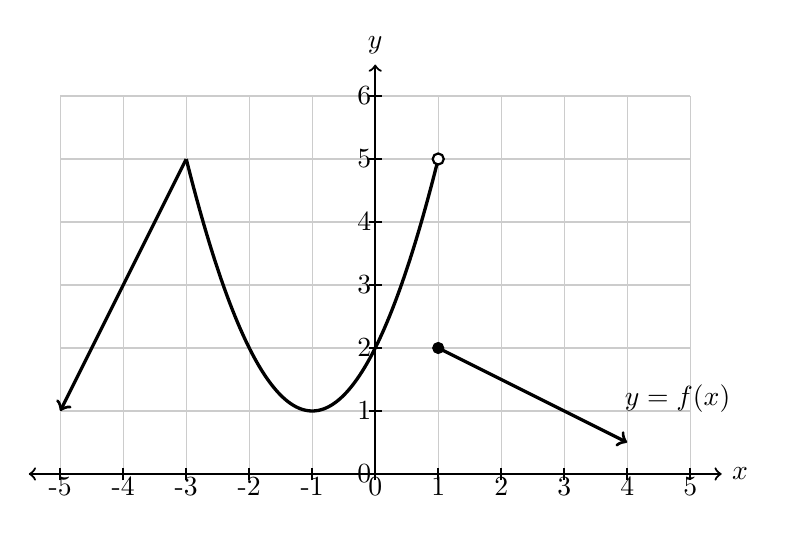
\begin{tikzpicture}[scale=.8]
\draw[gray!40] (-5, 0) grid[step=1] (5, 6);
\draw[<->,thick,black] (-5.5,0)--(5.5,0) node[right]{$x$};
\draw[->, thick,black] (0,0)--(0,6.5) node[above]{$y$};
\foreach \x in {-5,-4,...,5}
\draw[thick] (\x,-.1) --(\x,.1) node[below]{\x};
\foreach \y in {0,1,...,6}
\draw[thick] (-.1,\y) --(.1,\y) node[left] {\y};
\draw[domain=-5:-3,samples=100, very thick,<-] plot ({\x},{2*\x+11});
\draw[domain=-3:1,samples=100,very thick,-] plot ({\x},{(\x+1)^2+1});
\draw[domain=1:4,samples=100,very thick,->] plot ({\x},{-1/2*(\x-1)+2});
\draw[fill=white,thick] (1,5) circle[radius=0.25em];
\draw[fill=black] (1,2) circle[radius=0.25em];
\node at (4.8,1.2) {$y=f(x)$};
\end{tikzpicture}

\end{minipage}
\vfill

\end{parts}

\newpage




\question Suppose $f(x)$ is a continuous function whose derivative is
$f'(x)=-4(x-1)(x-2)^3(x+3)^2$.
\begin{parts}
\part[3] What are the critical numbers of $f(x)$?
\vspace{1in}
\part[5] Using a sign chart, find the intervals of increasing and decreasing for $f(x)$. Write your
answers using interval notation.

\vfill

\part[3] Classify each critical number as the location of a relative minimum, relative maximum, or
neither. No justification is needed.

\vspace{1.5in}
\end{parts}


\newpage




\question[11] On the axes below,
draw the graph of a function $f(x)$ which is \textbf{continuous} everywhere that satisfies all the
following conditions:

$f(-2)=0$ and $f(0)=3$. \medskip

$f(x)$ is not differentiable at $x=-2$. \medskip

$f'(x)>0$ on $(-2,0)$. \medskip

$f'(x)<0$ on $(-\infty, -2)\cup(0,\infty)$. \medskip

$f''(x)<0$ on $( -\infty,-2)\cup(-2,2)$. \medskip

$f''(x)>0$ on $( 2,\infty)$. \medskip

$\displaystyle \lim_{x\to \infty}f(x)=-1$.


\begin{center}
​      \begin{tikzpicture}[scale=1.2]
​      \draw[gray!60] (-6, -6) grid[step=1] (6, 6);
​      \draw[<->, thick,black] (-6.5,0)--(6.5,0) node[right]{$x$};
​      \draw[<->, thick,black] (0,-6.5)--(0,6.5) node[above]{$y$};
​      \foreach \x in {-6,-5,...,6}
​      \draw[thick] (\x,-.1) --(\x,.1)node[below]{\x};
​      \foreach \y in {-6,-5,...,6}
​      \draw[thick] (-.1,\y) --(.1,\y)node[left]{\y};
​      \end{tikzpicture}
\end{center}​




\newpage

\question[11] A woodworker finds that when they price their cutting boards at $\$50 $, they sell
$30$ cutting boards in a month. They determine that for each $\$1 $ price discount, they will sell
3 more cutting boards per month. If each cutting board costs $\$20$ to produce, find the price of
the cutting boards which will maximize their profit AND the number of cutting boards sold. Write
each answer clearly with units, and justify your solution gives the maximum profit. Show all
work.




\newpage

\question

\begin{parts}

\part[6] After $t$ weeks of practice, a typing student can type $120(1-e^{-0.3t})$ words per
minute. How long will it take for the student to be able to type 100 words per minute? Show all
work. You do not need to simplify your final answer, but include units.

\vfill




\part[6] A rich aunt wants to give her nephew $\$45,000$ when he turns 18. How much money
must she deposit in a trust fund paying $8\%$ compounded quarterly at the time of the
nephew's birth to yield $\$45,000$ when he turns 18? Show all work. You do not need to
simplify your answer.

\vfill

\end{parts}




\newpage

\question[8]
Find the inflection point(s) ($x$-value(s) only) and intervals of concavity for

$f(x)=9x^2-x^3+10x+12$. Give the intervals of concavity using interval notation. Show all work.

\newpage


\question[11] A dog daycare owner wants to build a rectangular fenced area along the side of
the daycare building, split into two equal parts by a fence parallel to one of its sides (see picture
below, the dashed lines denote fencing). If the side along the building needs no fence,
with 300 meters of fencing available to use, what dimensions for the outer rectangle will create
the largest total area? Show all work, including justification that your solution is optimal.

\begin{figure}[h]
​       ​       \begin{center}
​       ​       ​        \begin{tikzpicture}
​       ​       ​        ​       \draw[thick,dashed] (0,0) -- (6,0)--(6,4)--(0,4)--(0,0);
​       ​       ​        ​       \draw[thick,dashed] (3,0) --(3,4);
   \draw[ultra thick] (-2,0)--(8,0);
  % \foreach \x in {-2,-1,...,8}
   %\draw[thick] (\x,0) --(\x-0.25,-0.25);
\draw (3, -0.5) node {Building};
  \draw (0,4.2)--(6,4.2);
   \draw (0,4.1)--(0,4.3);
   \draw (6,4.1)--(6,4.3);
   \draw (6.2,0)--(6.2,4);
   \draw (6.1,0)--(6.3,0);
   \draw (6.1,4)--(6.3,4);
\draw (3,4.2) node[inner sep=2pt,fill=white] {$x$};
\draw (6.21,2) node[inner sep=2pt,fill=white] {$y$};
​       ​       ​        ​
​       ​       ​        ​
​       ​       ​        \end{tikzpicture}
​       ​       \end{center}
​       ​       %\caption{Useful figure for Problem 4}
​       \end{figure}

\newpage


\question Compute the following:

\begin{parts}

\part[5] Find $f'(x)$ if $f(x) = x^2\ln(4x).$ You do not need to simplify your final answer.

\vfill

\part[6] Find $g''(x)$ if $\displaystyle g(x)=e^{x^2+2x}$. You do not need to simplify your final
answer.

\vfill

\end{parts}

\newpage

\question

\begin{parts}
\part[6] For the demand function $D(p)=60-p^2$, find the elasticity of demand $E(p)$ and
evaluate it at $p=5.$ Show all work. You do not need to simplify your final numerical answer.

 \vfill




\part[5] Find the relative rate of change of $f(t)=t^3+2t$ at $t=3$. Show all work. You do not
need to simplify your final numerical answer.


\vfill
\end{parts}


\end{questions}

\end{document}
